\section{Diseño experimental y procedimientos}\label{sec:diseno}
Para garantizar una referencia verificable se define la función escalar \emph{sintética} en kilómetros locales:
\begin{align}
C_\star(x,y)=18&+20\exp\left[-\frac{(x-22)^2}{2(9)^2}-\frac{(y-28)^2}{2(11)^2}\right]\\
&+8\exp\left[-\frac{(x-49)^2}{2(6)^2}-\frac{(y-13)^2}{2(8)^2}\right]+3\sin(x/12)\cos(y/10).\label{eq:sintetica}
\end{align}
Se generan $n=24$ localizaciones uniformes aleatorias en $[1,59]\times[1,49]$ km, semilla 20261018, y observaciones $y_i=C_\star(s_i)+\varepsilon_i$ con $\varepsilon_i\stackrel{\mathrm{iid}}\sim N(0,1^2)\um$. Estos puntos \textbf{no son estaciones georreferenciadas}. Para RBF se declara $\ell=15$ km, $\lambda=0.05$ y $L=I$. Para IDW, potencia 2. Las reconstrucciones se evalúan en malla regular, pero el mapa de concentración estimada se enmascara fuera de la envolvente convexa de puntos simulados.

\subsection{Validación cruzada y evaluación de verdad conocida}
Se calcula el error dejando fuera una estación completa por turno: en cada uno de los $n$ pliegues, el interpolador se entrena sobre $n-1$ valores, sin reutilizar la observación eliminada. Las estadísticas son
\begin{equation}\RRMSE=\sqrt{\frac1n\sum_i(y_i-\widehat y_{-i})^2},\qquad\mathrm{MAE}=\frac1n\sum_i|y_i-\widehat y_{-i}|.\label{eq:rmse}\end{equation}
Como en el ensayo se conoce $C_\star$ en toda la malla, también se reporta el error de campo respecto a esa verdad, separando píxeles interiores y exteriores a la envolvente convexa. Este último cálculo \emph{no justifica extrapolar} en un estudio con datos reales.

\subsection{Ensayo dinámico}
Se utiliza $L=10\,000$ m, $u=1.5$ m/s, $D=10$ m$^2$/s, tiempo final $T=500$ s y refinamientos $N=24,48,96$ celdas por lado. $\Delta t$ se elige automáticamente para satisfacer \eqref{eq:cfl} con factor conservador de 0.6. Se compara el resultado con \eqref{eq:solucion}; la masa se mide como suma de volúmenes de celda.

\section{Resultados computacionales obtenidos}\label{sec:resultados}
Los resultados siguientes proceden de la ejecución de \texttt{src/validation/}\\\texttt{run\_synthetic\_experiments.py} y de doce pruebas automatizadas de Python. No se ejecutaron los programas MATLAB ni R porque los intérpretes no están instalados en el entorno. Es incorrecto afirmar que esas pruebas se completaron en MATLAB o R.

\begin{table}[H]\centering\caption{Reconstrucción del campo \emph{sintético}; concentraciones y errores en $\mu$g/m$^3$. Una sola semilla: 20261018.}\label{tab:recon}
\begin{tabular}{lrrr}\toprule
Método & RMSE LOOCV & RMSE interior & RMSE exterior \\\midrule
IDW (potencia 2) & 2.789 & 3.104 & 2.346 \\
RBF + Tikhonov ($\lambda=0.05$) & 2.533 & 2.558 & 2.552 \\\bottomrule
\end{tabular}\end{table}

En esta realización la RBF presenta menor RMSE tanto en estaciones retenidas como en el interior de la envolvente, pero no se extrapola esta diferencia a otras semillas, distribuciones, regímenes meteorológicos ni redes reales. El error sobre la zona exterior también es calculable gracias a la verdad sintética conocida, pero tales valores \emph{no} expresan confianza en extrapolaciones ambientales. En la ejecución, $\kappa_2(A)=3.94\times10^4$ para el diseño RBF de 24 estaciones; ello señala sensibilidad potencial sin regularización.

\begin{figure}[H]\centering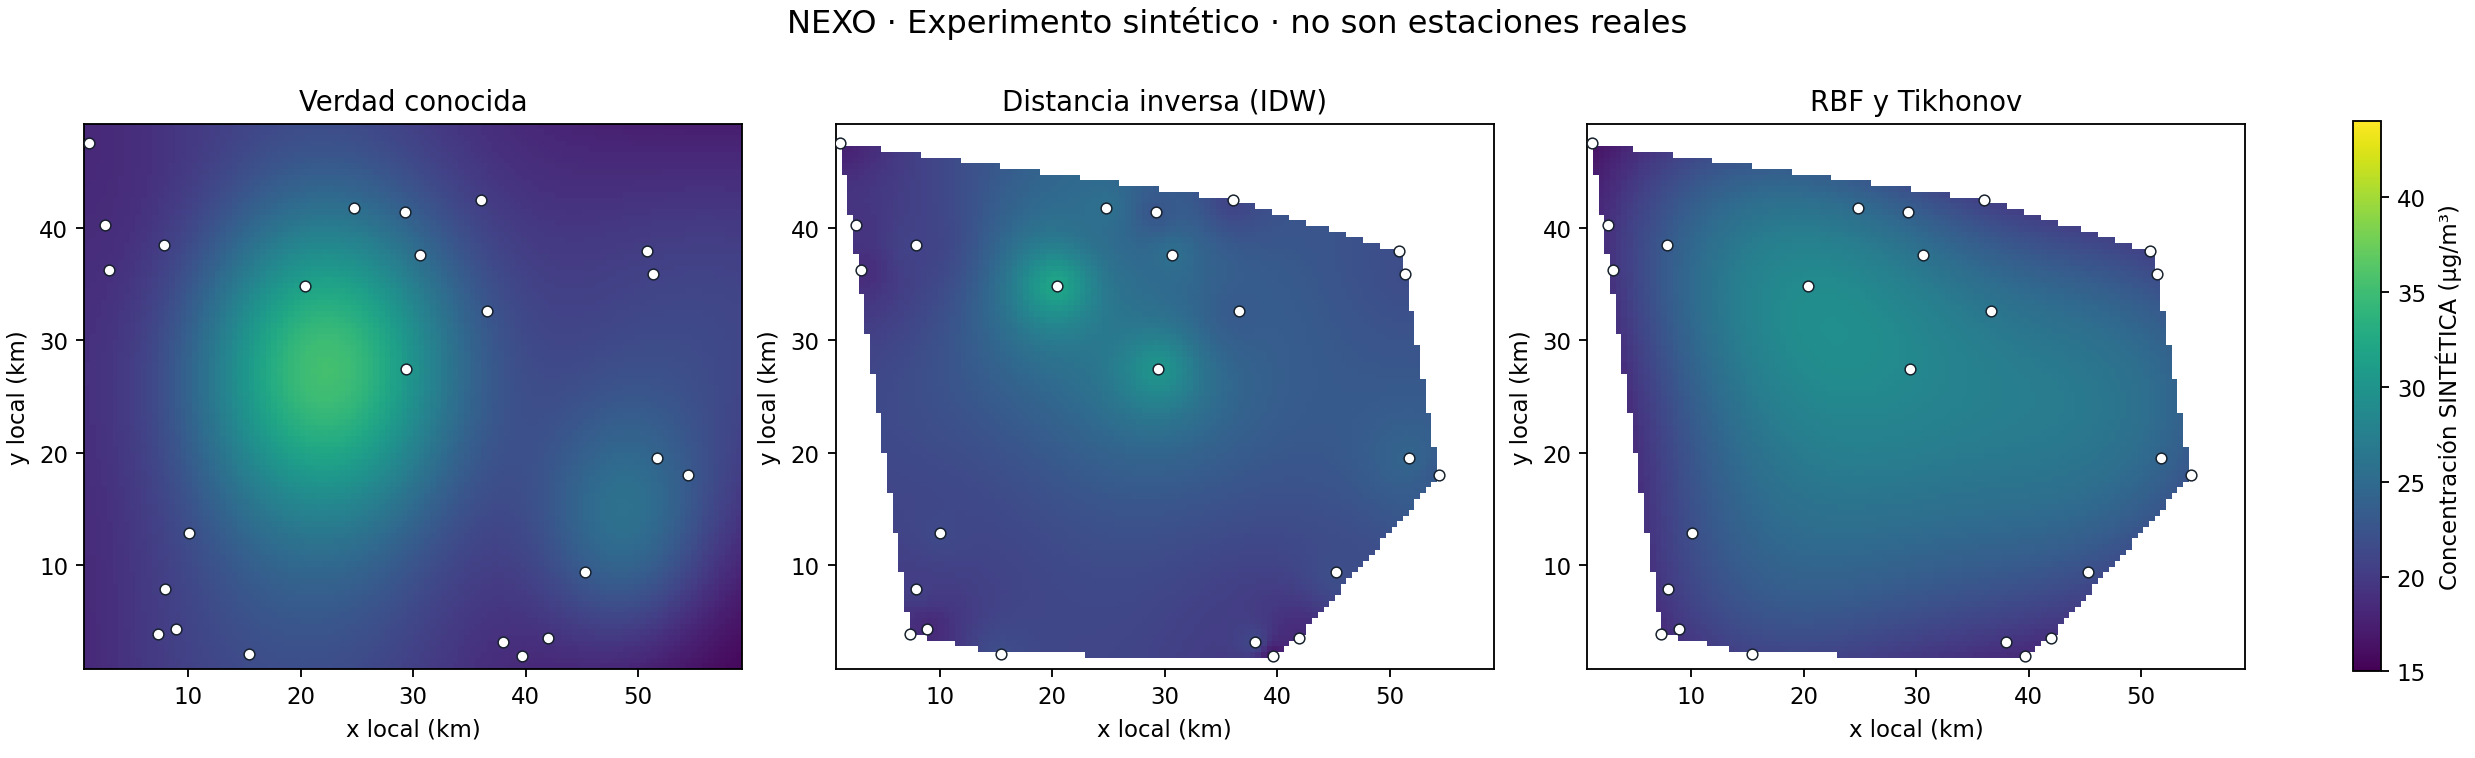
\includegraphics[width=\textwidth]{compare_synthetic.png}\caption{Comparación de la verdad conocida y reconstrucciones IDW y RBF regularizada. Puntos simulados; las dos reconstrucciones están enmascaradas fuera de la envolvente convexa. El dibujo no representa mediciones ni geografía real de Monterrey.}\label{fig:comparacion}\end{figure}

La figura \ref{fig:comparacion} vincula de forma visual los errores resumidos en la tabla \ref{tab:recon}. Debe enfatizarse que una menor desviación en promedio no equivale a recuperar la geometría de una pluma real o identificar fuentes.

\begin{figure}[H]\centering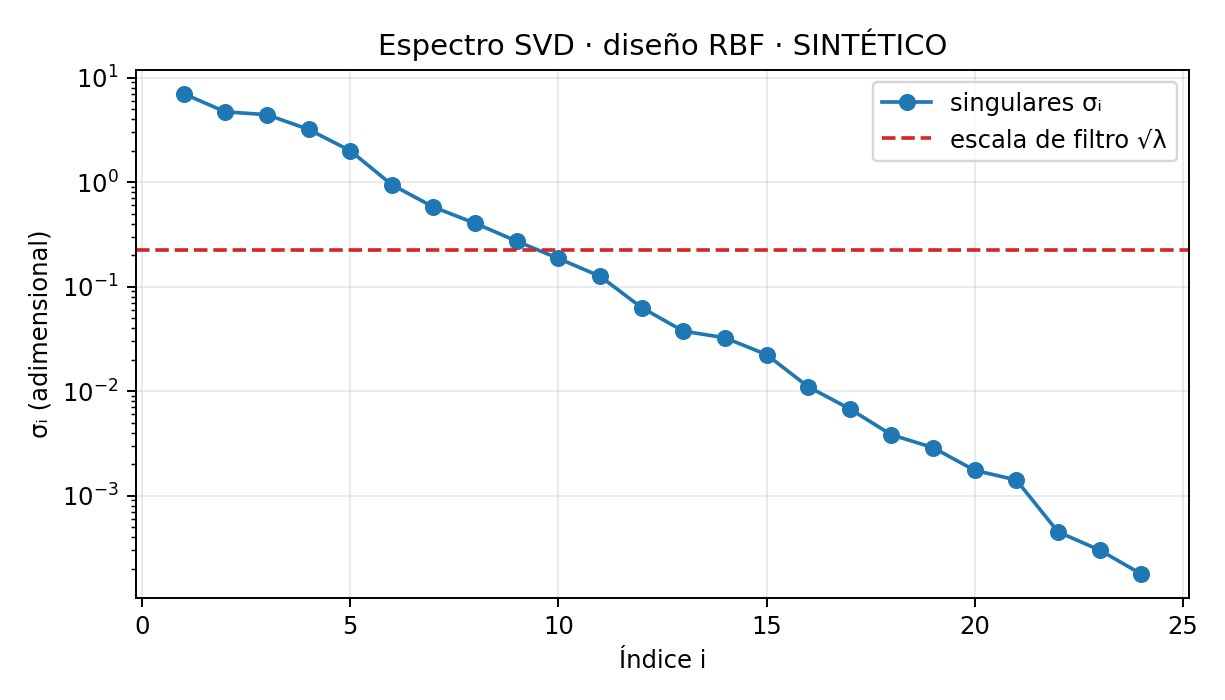
\includegraphics[width=.78\textwidth]{svd_synthetic.png}\caption{Espectro singular de la matriz de diseño RBF, con escala de referencia $\sqrt\lambda$. Experimento sintético.}\label{fig:svd}\end{figure}

La figura \ref{fig:svd} muestra por qué la separación entre valores singulares y el parámetro de penalización importa: las componentes de menor amplitud se vuelven vulnerables al ruido y la regularización reduce su peso, de acuerdo con \eqref{eq:filtros}.

\begin{figure}[H]\centering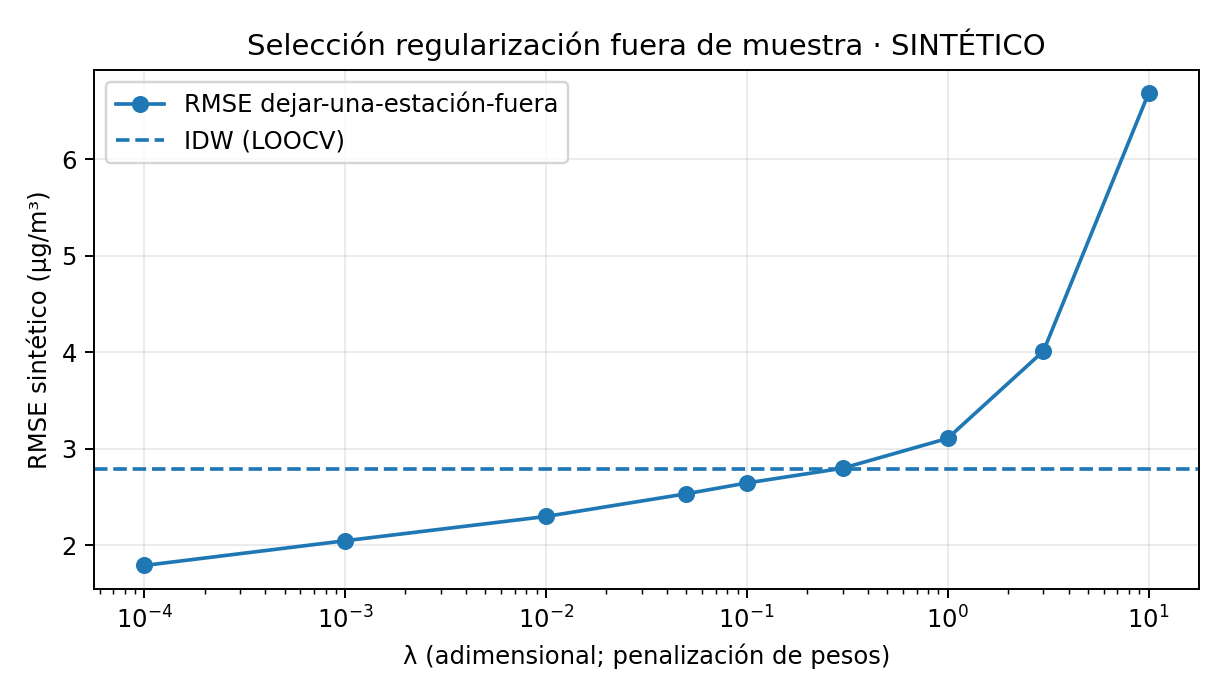
\includegraphics[width=.78\textwidth]{cv_synthetic.png}\caption{Barrido exploratorio de $\lambda$ y error al retener una estación por turno. No es validación anidada de la elección óptima de hiperparámetros.}\label{fig:cv}\end{figure}

La figura \ref{fig:cv} documenta explícitamente la dependencia respecto a $\lambda$; una selección posterior del mínimo de esta misma curva requeriría una evaluación externa adicional. El prototipo fija $\lambda=0.05$ antes de informar la métrica principal.

\subsection{Conservación y convergencia de la EDP}
\begin{table}[H]\centering\caption{Error RMS contra solución periódica analítica, \emph{simulación sintética}, $T=500$ s.}\label{tab:pde}
\begin{tabular}{rr}\toprule Celdas por eje & Error RMS ($\mu$g/m$^3$)\\\midrule 24 & 0.08326\\ 48 & 0.03705\\ 96 & 0.02104\\\bottomrule\end{tabular}\end{table}

\begin{figure}[H]\centering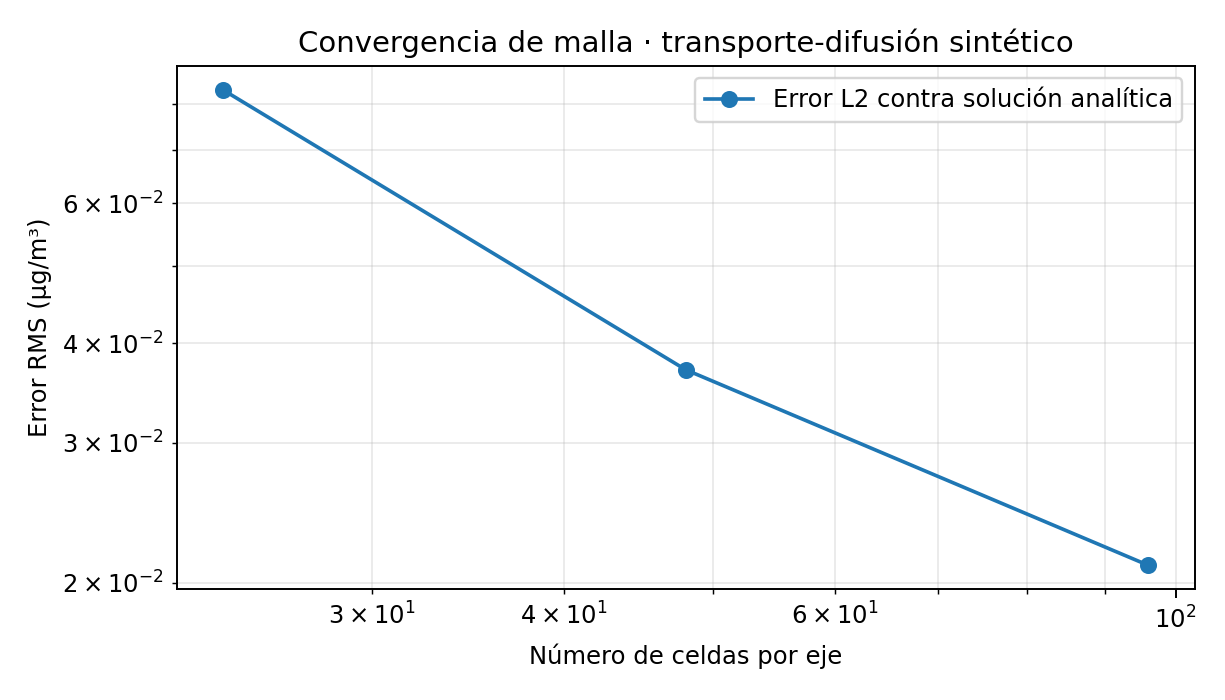
\includegraphics[width=.78\textwidth]{convergence_synthetic.png}\caption{Descenso del error RMS cuando se refina la malla en una ecuación con solución analítica conocida y fronteras periódicas.}\label{fig:convergencia}\end{figure}

La evolución en la tabla \ref{tab:pde} y figura \ref{fig:convergencia} es consistente con el esquema de transporte upwind de primer orden; no demuestra un orden de convergencia asintótico mediante solo tres resoluciones. La prueba aislada de conservación de masa, sobre un paso temporal con $50\times60$ celdas y datos aleatorios positivos, obtuvo diferencia relativa reportada igual a $0$ dentro de precisión de coma flotante. Este resultado numérico concuerda con la proposición \ref{prop:masa}; no significa ausencia de error de solución.

\subsection{Pruebas automatizadas y criterio de aceptación}
Doce pruebas Python terminaron sin fallos: semilla reproducible, coincidencia de IDW en puntos de observación, reconstrucción finita al eliminar estaciones, norma regularizada de coeficientes inferior a una opción casi no penalizada, matriz de rango conocido, gradiente de función afín, conservación de masa periódica, rechazo de paso de tiempo inestable, descenso de error por refinamiento de malla y consistencia elemental de RMSE/MAE. Otras dos pruebas comprobaron el flujo de proyección WGS84 a UTM y el rechazo de archivos de medición sin coordenadas. Estas pruebas verifican propiedades del código de referencia Python, \emph{no} ejecutan el código MATLAB ni comprueban paridad exacta MATLAB--R.
